\documentclass[twocolumn]{article}
\usepackage{algorithm}
\usepackage{algpseudocode}
\usepackage{enumitem}
\usepackage{amsmath}
\usepackage{array}
\usepackage{hyperref}
\usepackage{pgfplots}
\pgfplotsset{compat=1.18} % Set the compatibility version
\usepackage{booktabs} % For better-looking tables
% Adjust the page margins if needed
\usepackage[margin=1in]{geometry}
\usepackage{multirow}
\usepackage{siunitx}
% Set the document title, author, and date
\title{\textbf{A Comparative Analysis of Insertion Sort and Quick Sort Algorithms in C++, Java, and Python} }
\author{
   \textbf{Paper Work: Taki Tamim -200302} \\
% \vspace{20pt}
 \hspace{70pt} \textbf{Fazle Rabbi-200304}\\
 \hspace{30pt}\textbf{Formatting: Moloy Kumar Das-2003012}\\
 \vspace{20pt}
\hspace{130pt}\textbf{Rakibul Hasan Durjoy-2003018}\\
\hspace{40pt}\textbf{Slide maker:}\hspace{5pt}\textbf{Md. Rashedul Islam -2003024}\\
\vspace{20pt}
\hspace{150pt}\textbf{Md. Shefat Hossen Shoikat-2003045}\\
}
\date{\textbf{\today}}

\begin{document}
\maketitle

%\begin{abstract}
\section{Abstract}
	The significance of algorithms in software and programming demands an understanding of the fundamental ideas that underlie them. We often meet issues in our daily lives that require us to start the data sorting process to find solutions. A significant amount of programming logic has been developed for both the case and the generic case. The authors of this study used bubble sort and Tim sort as their two techniques of sorting. C++ is used in the construction of the sorting program. To solve a problem more quickly and effectively while using minimal resources, algorithms are needed.
%\end{abstract}


\section{Introduction}
Sorting algorithms play a crucial role in computer science as they help efficiently organize and process data.\cite{1} This paper focuses on comparing two sorting algorithms, namely insertion sort and quick sort, implemented in three popular programming languages: C++, Java, and Python. Our main objective is to evaluate their performance by measuring execution time and identify factors that affect their efficiency across programming environments. While Insertion Sort was developed using iterative programming approaches, Quick Sort was implemented utilizing recursive programming approaches.\cite{1} \cite{2}The programming language options were divided into groups according to: \\
\textbf{KeyWord:}Sorting Algorithms, Insertion Sort, Quick Sort, Performance Analysis, C++, Java, Python, Programming Languages

\begin{enumerate}
	\item Virtual machine-based languages: Java (compiled and interpreted language)
	\item Native Languages: C++ (Compiled language)
	\item Scripting Languages: Python (Interpreted language)\cite{3}
  \end{enumerate}

  \vspace{20pt}
  \section*{The key goals of this study are:}
  
  \begin{enumerate}
	  \item \textbf{Implementing both Algorithm:}
	  Implement the sorting algorithms in C++, Java, and Python to ensure a basis for comparison.
	  
	  \item \textbf{Conducting performance analysis:}
	  Measure execution times for various sizes of input arrays to conduct a thorough performance analysis.
	  
	  \item \textbf{Investigating language and strategy impact:}
	  Investigate how the choice of programming language and implementation strategies impact the performance of the algorithms.
	  
	  \item \textbf{Identifying scenarios for performance differences:}
	  Identify scenarios where one algorithm may outperform the other based on data characteristics and programming environments.
	  
	  \item \textbf{Providing insights and recommendations:}
	  Provide insights and recommendations for developers to make informed decisions when selecting and implementing sorting algorithms in their applications.
  \end{enumerate}
  
  %The key goals of this study are:\hspace{10pt}
  %\begin{itemize}
   %   \item Implementing both algorithms in C++, Java, and Python to ensure a basis for comparison.
	%\item Conducting a performance analysis by measuring execution times for sizes of input arrays.
	%\item Investigating how the choice of programming language and implementation strategies impact algorithm performance.
	%\item Identifying scenarios where one algorithm may outperform the other based on data characteristics and programming environments.
	%\item Providing insights and recommendations for developers to make decisions when selecting and implementing sorting algorithms in their applications.
  %\end{itemize}
  
  \vspace{20pt}
  \section*{We anticipate that this research will:}
  \begin{enumerate}
	\item Illuminate the strengths and weaknesses of insertion sort and Quick sort across programming languages.
	
	\item Offer guidance to developers on optimizing sorting algorithms based on use cases and performance requirements.
	
	\item Contribute to an understanding of algorithm design and implementation choices for data management.
  \end{enumerate}
  \cite{2}\cite{3}\cite{4}
%close introduction
\section{Background Study}
A straightforward and natural sorting method called "insertion sort" builds the sorted array one element at a time. For small data sets, especially those that have been significantly sorted, it is simple to apply and highly effective. Insertion sort operates by assuming that the initial item in the array is already sorted. It then compares the second item to the first. If the first item is larger, the second is placed ahead of it. These steps ensure that the first two items are sorted. The third item is then compared to the ones on its left, and it is positioned after the item that is smaller. If there is no smaller item, the third item should be inserted at the beginning of the array. This procedure continues until the entire array is sorted.

\vspace{30pt}
\begin{algorithm}
  \caption{Insertion Sort}
  \begin{algorithmic}[1]
  \Procedure{InsertionSort}{$arr, n$}
      \For{$i \gets 1$ \textbf{to} $n-1$}
          \State $key \gets arr[i]$
          \State $j \gets i - 1$
          \While{$j \geq 0$ \textbf{and} $arr[j] > key$}
              \State $arr[j + 1] \gets arr[j]$
              \State $j \gets j - 1$
          \EndWhile
          \State $arr[j + 1] \gets key$
      \EndFor
  \EndProcedure
  \end{algorithmic}
  \end{algorithm}
  
%\textbf{Pseudo-code:}\hspace{30pt}// Insertion Sort
%\vspace{5pt}

%\begin{verbatim}
%for i = 1 to n-1
 %   key = A[i]
  %  j = i - 1
   % while j >= 0 and A[j] > key
    %    A[j + 1] = A[j]
     %   j = j - 1
    %A[j + 1] = key
%\end{verbatim}
The time complexity of insertion sort varies under different scenarios. In the best case, when the array is already sorted, the algorithm only needs to compare each element with its predecessor, requiring n steps to sort the n-element array. The inner loop does not run at all when the array has already been sorted, but the outside loop continues for n times. Thus, the number of comparisons is limited to n. Complexity is hence linear. On the other hand, in the worst case, when the array is reverse-sorted, insertion sort has to insert each element at the beginning of the sorted subarray, resulting in a time complexity of $O(n^2)$. In the average case, where the array elements are in random order, the running time is approximately $O(n^2 / 4) = O(n^2)$. Since every element must be compared to every other element, (n-1) comparisons are conducted for every nth element. Consequently, $n \times (n-1)$ is the total number of comparisons.

\vspace{20pt}
Regarding space complexity, insertion sort uses a constant amount of additional variables besides the input array, resulting in a space complexity of $O(1)$.\vspace{20pt}
\vspace{5pt}
Among the quickest and best sorting algorithms are Bubble Sort, Selection Sort, and Insertion Sort. The Quick Sort Algorithm was created by renowned computer scientist C.A.R. Hoare. The Quick Sort algorithm is another excellent illustration of the divide and conquer tactic in action.\cite{5}\vspace{30pt}

The fundamental ideas behind the Quick Sort algorithm are as follows:\vspace{20pt}

    -$>$Select the pivot element from the array that has to be sorted.\vspace{10pt}

    -$>$To see that every element in the array with a value smaller than the pivot appears before it, and every element in the array with a value larger than the pivot appears after it, do a partition operation. Following this procedure, the pivot is in the array's final location.\vspace{10pt}

    -$>$The sublist of larger entries and the sublist of smaller elements are sorted recursively.\cite{5}
%close 3rd page
\vspace{20pt}
\begin{algorithm}
  \caption{Partition Function of Quick Sort}
  \begin{algorithmic}[1]
  \Procedure{PlacePivot}{$arr, low, high$}
      \State $pivot \gets arr[high]$
      \State $i \gets low - 1$
      \For{$j \gets low$ to $high - 1$}
          \If{$arr[j] \leq pivot$}
              \State $i \gets i + 1$
              \State Swap $arr[i]$ and $arr[j]$
          \EndIf
      \EndFor
      \State Swap $arr[i + 1]$ and $arr[high]$ \Comment{Place pivot in its final position}
      \State \textbf{return} $i + 1$ \Comment{Return the index of the pivot}
  \EndProcedure
  \end{algorithmic}
  \end{algorithm}
  
%\textbf{Partition Function of Quick Sort:}
%\begin{verbatim}
%function partition(arr, low, high)
 %   pivot = arr[high]
  %  i = low - 1

   % for j = low to high - 1
    %    if arr[j] <= pivot
     %       i = i + 1
      %      swap(arr[i], arr[j])

    %swap(arr[i + 1], arr[high])
    %return i + 1
%\end{verbatim}
\vspace{10pt}

%Here is the working principle of the Partition function:
%\begin{itemize}
 % \item Choose a pivot: In general, the first element, a random element, or the last element of the sample is selected as the pivot.
  %\item Set up pointers: Two pointers, which are named as low and high, are initialized at the beginning and end of the array that is going to be partitioned.
  %\item Iterate and swap: The algorithm iterates through the array, comparing elements with the pivot and swapping them based on the below:
   % \begin{itemize}
    %  \item If an element at low is larger than or equal to the pivot, swap it with the element at high, and decrement high.
     % \item Otherwise, increment low.
    %\end{itemize}
%\end{itemize}

\section*{Here is the working principle of the Partition  function:}

\begin{enumerate}[label=\textbf{\arabic*.}, left=0pt, itemsep=0.5em]
    \item \textbf{Choose a pivot:}
    In general, the first element, a random element, or the last element of the sample is selected as the pivot.
    
    \item \textbf{Set up pointers:}
    Two pointers, named as low and high, are initialized at the beginning and end of the array that is going to be partitioned.
    
    \item \textbf{Iterate and swap:}
    The algorithm iterates through the array, comparing elements with the pivot and swapping them based on the following:
    
    \begin{itemize}
        \item If an element at low is larger than or equal to the pivot, swap it with the element at high, and decrement high.
        \item Otherwise, increment low.
    \end{itemize}
    
    \item \textbf{Place pivot in position:}
    When low and high pointers meet, swap the pivot with the element at high. This places the pivot in its final sorted position, with smaller elements to its left and larger elements to its right. Also, return the index of high as that is needed in the main algorithm, which is used to find the particular index number.
\end{enumerate}
%close 4th page
\vspace{10pt}
The Main Algorithm of Quick Sort is below:
\begin{algorithm}
  \caption{ Quick Sort Function}
  \begin{algorithmic}[1]
  \Procedure{QuickSort}{$arr, low, high$}
      \If{$low < high$}
          \State $pivotIndex \gets$ \Call{Partition}{$arr, low, high$}
          \State \Call{QuickSort}{$arr, low, pivotIndex - 1$} \Comment{Sort the left subarray}
          \State \Call{QuickSort}{$arr, pivotIndex + 1, high$} \Comment{Sort the right subarray}
      \EndIf
  \EndProcedure
    \end{algorithmic}
  \end{algorithm}
  
  \section*{Complexity Analysis of Quick Sort by Iteration}

\begin{center}
\begin{tabular}{|c|c|c|}
\hline
\textbf{Iteration} & \textbf{Size of Subarray} & \textbf{Work Done } \\
\hline
0 & $n$ & $O(n)$ \\
1 & $\frac{n}{2}$ (on average) & $O(n)$ \\
2 & $\frac{n}{4}$ (on average) & $O(n)$ \\
3 & $\frac{n}{8}$ (on average) & $O(n)$ \\
\vdots & \vdots & \vdots \\
$k$ & $\frac{n}{2^k}$ (on average) & $O(n)$ \\
\hline
\end{tabular}
\end{center}

The total work done is the sum of the work done in each iteration:

\[
T(n) = O(n) + O(n) + \ldots + O(n) = k \cdot O(n)
\]

To find the number of iterations ($k$), we solve the following equation:

\[
\frac{n}{2^k} = 1 \implies k = \log_2 n
\]

Therefore, the overall time complexity is:

\[
T(n) = O(n \log n)
\]
%close 5th page 
\section*{The time complexity of Quick Sort is analyzed in terms of the number of comparisons and swaps.
}
\subsection*{Best Case:}

In the best case, the pivot chosen is always the median element. In each partitioning step, the array is divided into two equal halves. Therefore, the recurrence relation for the best-case time complexity is given by:

\[
T(n) = 2 \cdot T\left(\frac{n}{2}\right) + O(n)
\]

By solving the recurrence relation, we find that the best-case time complexity of Quick Sort is $O(n \log n)$.

\subsection*{Average Case:}

On average, if the pivot is chosen randomly, the expected time complexity is also $O(n \log n)$. The recurrence relation remains the same as in the best case.

\subsection*{Worst Case:}

In the worst case, the pivot is always the smallest or largest element. This leads to an unbalanced partition, and the recurrence relation becomes:

\[
T(n) = T(n-1) + O(n)
\]

Solving this recurrence relation yields the worst-case time complexity of $O(n^2)$.

\subsection*{Space Complexity:}

The space complexity of Quick Sort is dominated by the recursive call stack. In the worst case, the maximum depth of the call stack is $\log_2 n$, resulting in a space complexity of $O(\log n)$.
%close background Study
\cite{1}\cite{6}\cite{7}
\section{Result \& Analysis}
The experiments were carried out on a system with the same configuration, running on MacBook Pro. The sorting algorithms were executed on an M2 MacBook Pro, which had 16GB RAM and an M2 chip.
\subsection*{Data Table:}
\begin{table}[h]
  %\centering
  \begin{tabular}{|c|c|c|}
    \hline
    \multirow{2}{*}{Element} & Time for Insertion  & Time for Quick \\
    & sort(\si{\micro\second}) & sort(\si{\micro\second}) \\
    \hline
    10 & 85 & 138 \\
    \hline
    100 & 1257 & 1458 \\
    \hline
    1000 & 7580 & 8585 \\
    \hline
    10000 & 14312 & 12917 \\
    \hline
    100000 & 72819 & 54659 \\
    \hline
  \end{tabular}
  \caption{Testing For C++ Language}
  \vspace*{0.8cm}
\end{table}


%\vspace{300pt}
\begin{figure}[t]
	%\centering
	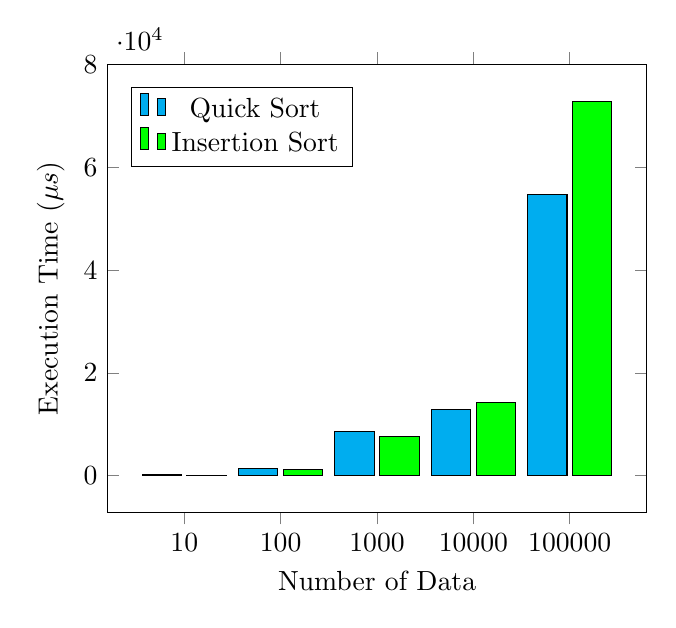
\begin{tikzpicture}
	  \begin{axis}[
		ybar,
		bar width=0.50cm,
		xlabel={Number of Data},
		ylabel={Execution Time ($ \mu s $)},
		symbolic x coords={10, 100, 1000, 10000, 100000},
		xtick=data,
		legend style={at={(0.25,0.95)},anchor=north},
		enlarge x limits={0.2},
	  ]
  
	  \addplot[fill = cyan] coordinates {(10,138) (100,1458) (1000,8585) (10000,12917) (100000,54659)};
		\addlegendentry{Quick Sort}
		\addplot[fill = green] coordinates {(10,85) (100,1257) (1000,7580) (10000,14312) (100000,72819)};
		\addlegendentry{Insertion Sort}
  
	  \end{axis}
  
	\end{tikzpicture}
  
	\caption{Comparison between Insertion and Quick Sort in C++ Language}
  \end{figure}  

  \begin{table}[h]
    %\centering
    \begin{tabular}{|c|c|c|}
      \hline
      \multirow{2}{*}{Element} & Time for Insertion  & Time for Quick \\
      & sort(\si{\micro\second}) & sort(\si{\micro\second}) \\
      \hline
      10 & 474 & 614 \\
      \hline
      100 & 5697 & 7805\\
      \hline
      1000 & 44289 & 35644 \\
      \hline
      10000 & 66598 & 46016 \\
      \hline
      100000 & 256741 & 187876 \\
      \hline
    \end{tabular}
    \caption{Testing For Python Language}
  \end{table}


  \begin{figure}
    %\centering
    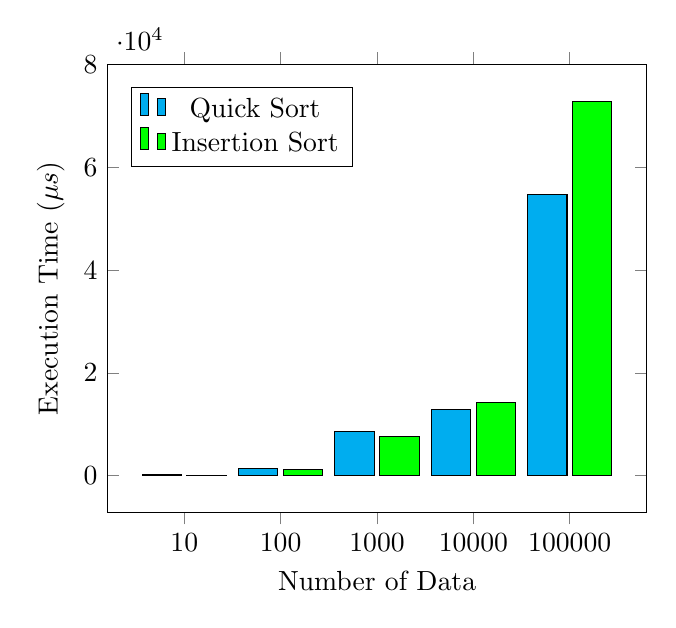
\begin{tikzpicture}
      \begin{axis}[
      ybar,
      bar width=0.50cm,
      xlabel={Number of Data},
      ylabel={Execution Time ($ \mu s $)},
      symbolic x coords={10, 100, 1000, 10000, 100000},
      xtick=data,
      legend style={at={(0.25,0.95)},anchor=north},
      enlarge x limits={0.2},
      ]
    
      \addplot[fill = cyan] coordinates {(10,138) (100,1458) (1000,8585) (10000,12917) (100000,54659)};
      \addlegendentry{Quick Sort}
      \addplot[fill = green] coordinates {(10,85) (100,1257) (1000,7580) (10000,14312) (100000,72819)};
      \addlegendentry{Insertion Sort}
    
      \end{axis}
    
    \end{tikzpicture}
    
    \caption{Comparison between Insertion and Quick Sort in Python Language}
    \end{figure}  
  
  
\clearpage
% % here graph will be added
\section*{Theoretical Background and Practical Results}

From the theoretical background, we can see that the time complexity of Insertion Sort is $O(N^2)$ in the worst case and $O(N)$ in the best case. As far as space complexity is concerned, it is always constant, $O(1)$.

For Quick Sort, the average time complexity is $O(N \log N)$, which rises up to $O(N^2)$ in the worst-case scenario. This happens when the array is already sorted in reverse. The space complexity of the Quick Sort algorithm is $O(\log N)$.

Relating the results from practical data, we observe that for a smaller size of data (i.e., 100), Insertion Sort performs better than Quick Sort, while for a larger dataset (i.e., 100,000), Quick Sort performs better. For a sorted dataset, the Insertion Sort algorithm outperforms the Quick Sort. This remains true for any amount of dataset.

Discussing the dependency on language, we observe that Python takes more time to implement even though it follows the theoretical aspects of Insertion and Quick Sort. This may be because Java and C++ are statically typed languages. On the other hand, Python is a dynamically typed language.

Python is easier to understand and read. It also requires fewer lines of code to implement these algorithms compared to both C++ and Java. However, for more computing efficiency, using C++ or Java is recommended, as there is a tiny difference between them when it comes to execution speed.
\vspace{100pt}


\section{Conclusion}
Conducting this research, we understand that insertion sort outperforms quicksort when the dataset is tiny, but quicksort performs far better for a huge dataset (i.e., 100000). Insertion sort is a better choice for a sorted dataset since, in this case, it provides linear time complexity. However, for quicksort, it becomes quadratic complexity. This rule is followed by any type of programming language, even though different programming languages take different spans of time to implement it.

One of the major drawbacks of this experiment is that it was conducted only on a MacBook Pro. It would be better if we could perform this experiment on various hardware configurations and different operating systems (i.e., Windows, Linux). This can be improved not only by using a comparatively more lower-level language (like assembly) but also by using some modern-level languages like JavaScript, Rust. This will create more diversified results. We can also improve it by using more data points, which will help us visualize the time-taking trend by these two algorithms more clearly.
\section{References:}
\bibliography{mybib.bib}
\bibliographystyle{ieeetr}




% % Add your bibliography here
% % \bibliographystyle{plain}
% % \bibliography{your_bibliography_file}

\end{document}
